\chapter{Analyse}
\label{sec:analyse}
Zusätzlich zu den maschinellen Lernkomponenten stellt Unity auch Demonstrationsumgebungen bereit, in denen verschiedene Lösungen für gängige Verstärkungslernprobleme implementiert sind. In der Walker-Demo wird ein physisch simulierter Charakter darauf trainiert, zu einem Zielwürfel zu laufen. Sie implementiert bereits einige grundlegende Steuerungsmechanismen, die erforderlich sind, um einen Charakter in einer Umgebung zu bewegen und zu kontrollieren. Aus diesem Grund wird in dieser Arbeit die Walker-Demo als Basis für die Entwicklung genutzt. 

In diesem Kapitel wird daher die Walker-Demo analysiert, um in den folgenden Kapiteln darauf aufzubauen. Es wird untersucht wie die Lernumgebung aufgebaut ist. Anschließend wird der Ablauf und die Komponenten für das verstärkende Lernen analysiert. Zum Abschluss wird das Trainingsergebnis und die Bewegungsabläufe der Demo analysiert.
\section{Lernumgebung}
Die Umgebung besteht aus einem quadratischen Spielfeld mit einem Boden und Wänden, die der Charakter nicht verlassen kann (siehe Abbildung \ref{fig:walker_aufbau}). Diese Begrenzungen dienen dazu, die Bewegung des Charakters zu kontrollieren und sicherzustellen, dass die Lernumgebung konsistent bleibt. Die Umgebung umfasst weiterhin den Läufer und das Ziel.

\begin{figure}[H]
  \centering  
  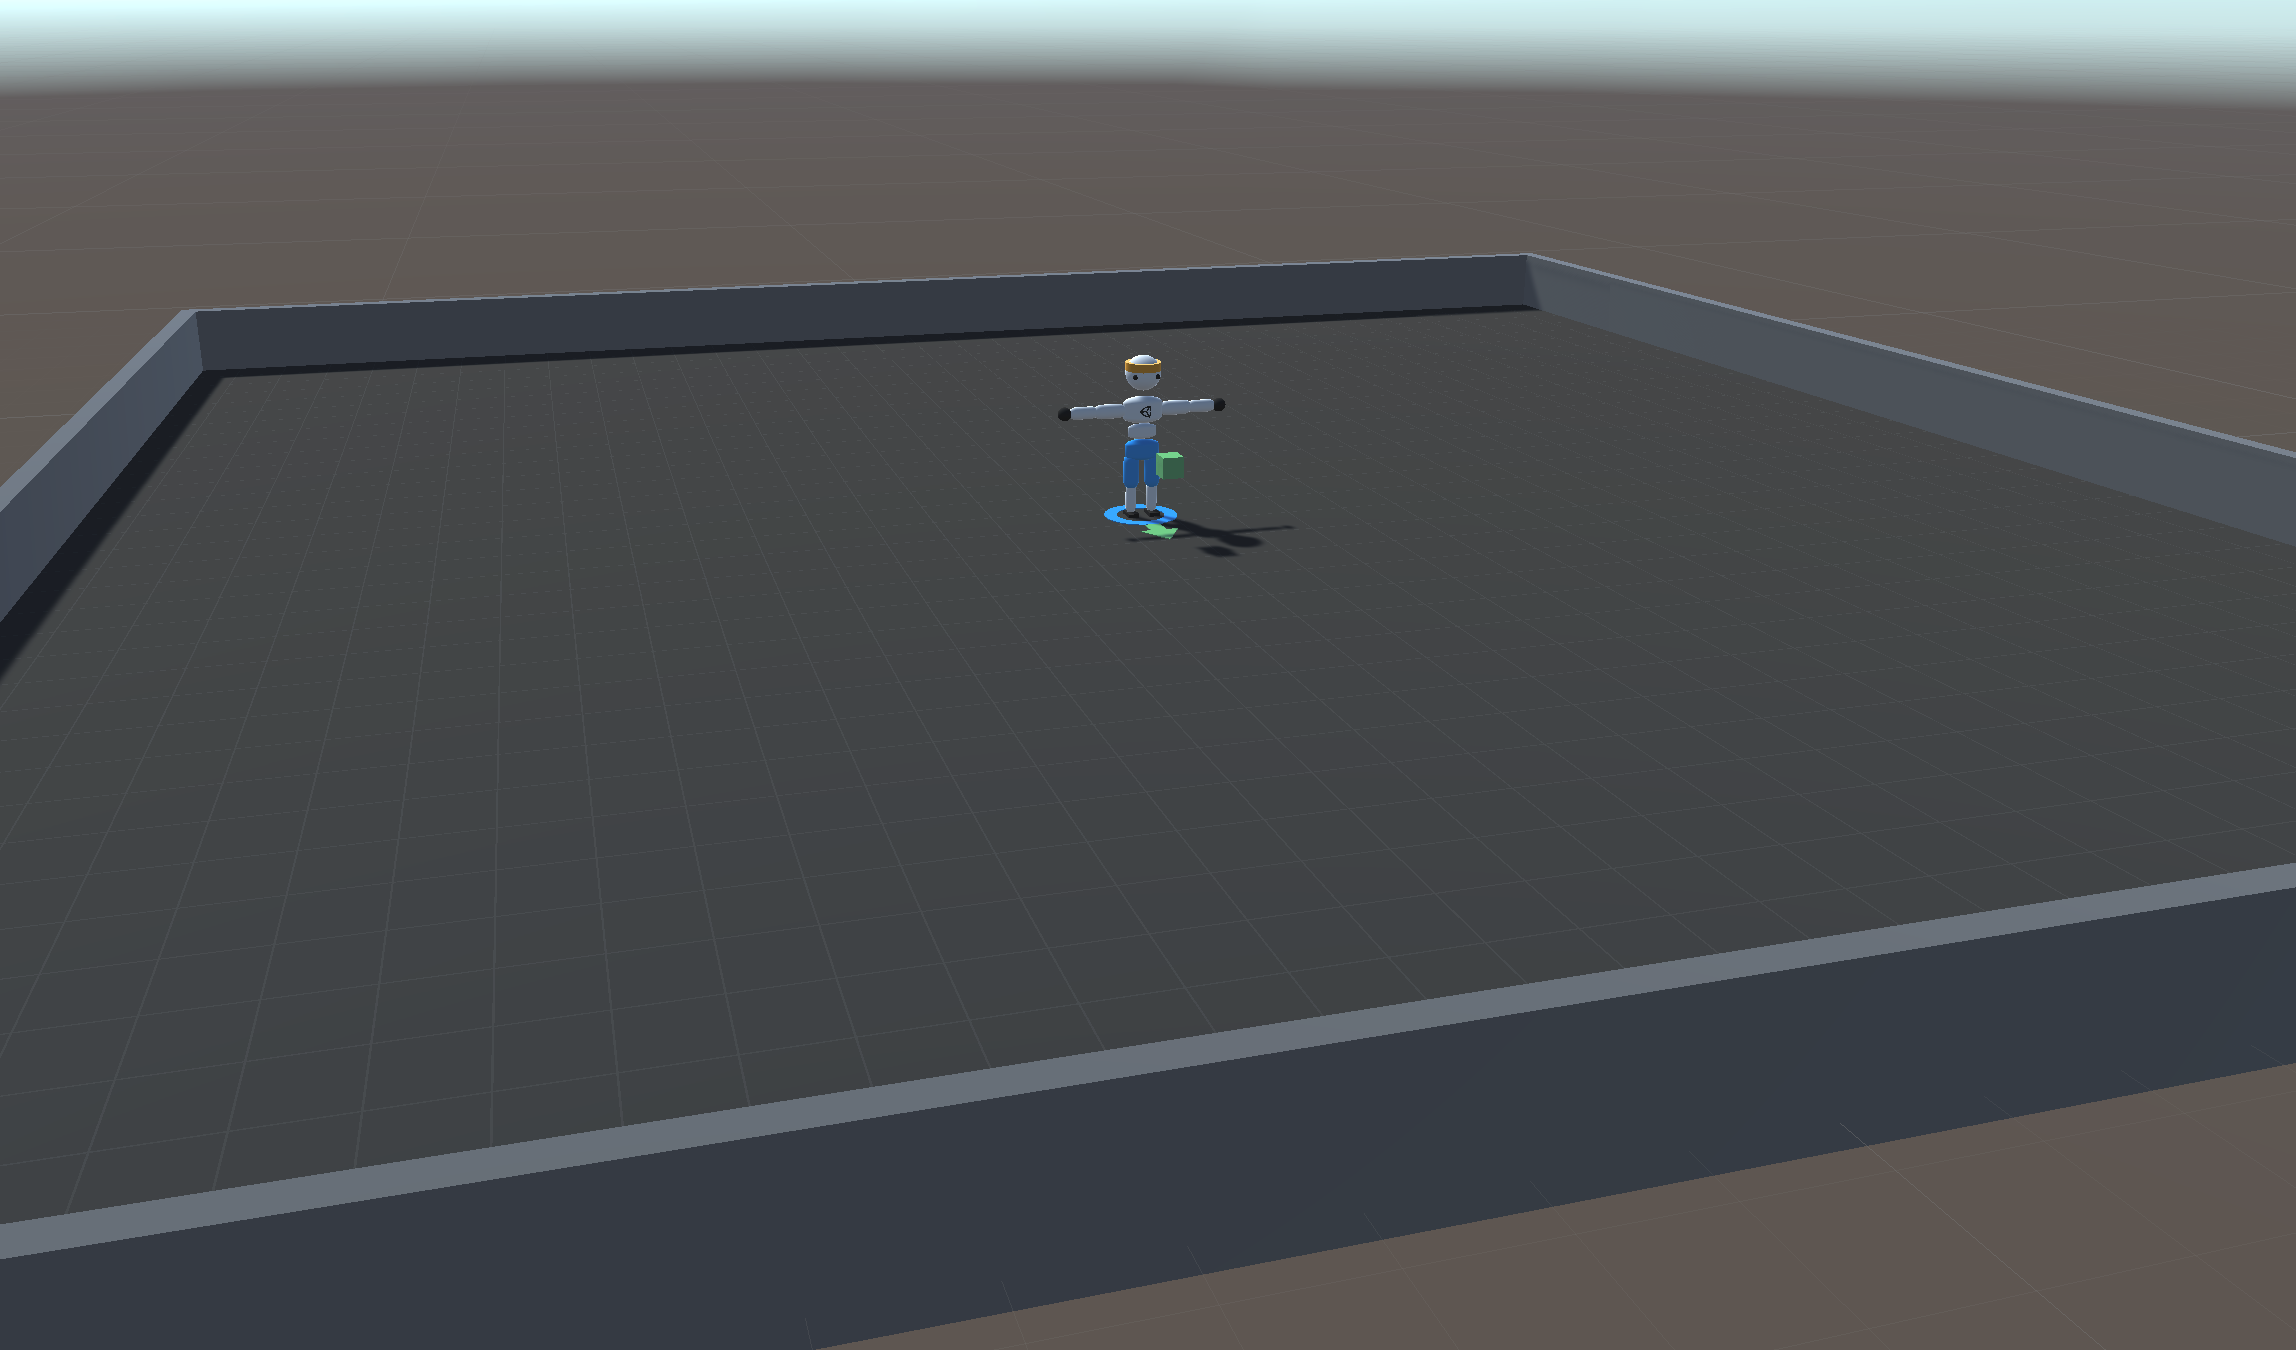
\includegraphics[scale=0.35]{img/walker_aufbau.png}
  \caption{Walker-Demo Umgebung}
  \label{fig:walker_aufbau}
\end{figure}

Der Läufer besteht aus einfachen geometrischen Körpern. Insgesamt 11 Kapseln, drei Kugeln und zwei Quadern von welchen jede über eine Festkörper- und eine Kollisions-Physikkomponente verfügt. Die Gelenke zwischen den Körperteilen werden als Kugelgelenke simuliert, um eine flexible und natürliche Bewegung zu gewährleisten. Die genaue Physikkonfiguration der Körperteile wird in der Tabelle \ref{table:walker_körperteile} veranschaulicht. Diese Konfiguration spielt eine zentrale Rolle, da die gesetzten Freiheiten sowie Einschränkungen beeinflussen wie der Läufer lernt, auf das Ziel zuzulaufen.

\begin{figure}[H]
  \centering  
  \includegraphics[scale=0.35]{img/läufer.png}
  \caption{Walker-Demo Läufer}
  \label{fig:läufer}
\end{figure}

\begin{table}[H]
  \centering
  {\rowcolors{1}{gray!10}{white}
  \begin{tabular}{ |p{3cm}|p{3cm}|p{2cm}|p{4cm}|p{2cm}| }
  \hline
  \textbf{Körpertei}l& \textbf{Verbundenes Körperteil} & \textbf{Gewicht} & \textbf{Winkellimits} & \textbf{Form} \\
  \hline
  Hüfte & - & 15kg & - & Kapsel \\
  \hline
  Wirbelsäule & Hüfte & 10kg & x(-20,20) y(-20,20) z(-15,15) & Kapsel \\
  \hline
  Oberkörper & Wirbelsäule & 8kg & x(-20,20) y(-20,20) z(-15,15) & Kapsel \\
  \hline
  Kopf & Oberkörper & 6kg & x(-30,10) y(-20,20) & Kugel \\
  \hline
  Oberarm LR & Oberkörper & je 4kg & x(-60,120) y(-100,100) & Kapsel \\
  \hline
  Unterarm LR & Oberarm & je 3kg & x(0,160) & Kapsel \\
  \hline
  Hand LR & Unterarm & je 2kg & - & Kugel \\
  \hline
  Oberschenkel LR & Hüfte & je 14kg& x(-90,60) y(-40,40) & Kapsel \\
  \hline
  Unterschenkel LR & Oberschenkel & je 7kg &  x(0,120) & Kapsel \\
  \hline
  Fuß LR & Unterschenkel & je 5kg & x(-20,20) y(-20,20) z(-20,20) & Quader \\
  \hline
  \end{tabular}}
  \caption{Walker Agent Körperteile}
  \label{table:walker_körperteile}
\end{table}

Das Walker Agent Skript, definiert den Läufer als Agent für das maschinelle Lernen. In Abbildung \ref{fig:agent_konfiguration} wird die Agentenkomponente im Inspektor gezeigt. Diese Komponente ist entscheidend für die Konfiguration des Läufers. Um die Komponente zu nutzen, müssen hier die Körperteile des Walkers referenziert werden. Das Walker Agent Skript registriert die Körperteile bei der Initialisierung in der Gelenk Motor Steuerung, wodurch eine effektive Schnittstelle zur Kontrolle der Gelenke geschaffen wird. Die Gelenk Motor Einstellungen (Joint Drive Settings) siehe Abbildung \ref{fig:agent_konfiguration} \hl{bestimmen die Stärke mit welcher die Gelenke in die Zielstellung bewegt werden.} Zusätzlich kann eine Zielgeschwindigkeit festgelegt werde und ob die Geschwindigkeit variieren soll während dem Training. Die Geschwindigkeit während dem Training zu variieren hilft dem Agent sein Verhalten besser an Umgebungsveränderungen anzupassen. Als letztes muss auch das Zielobjekt referenziert werden.

\begin{figure}[H]
  \centering  
  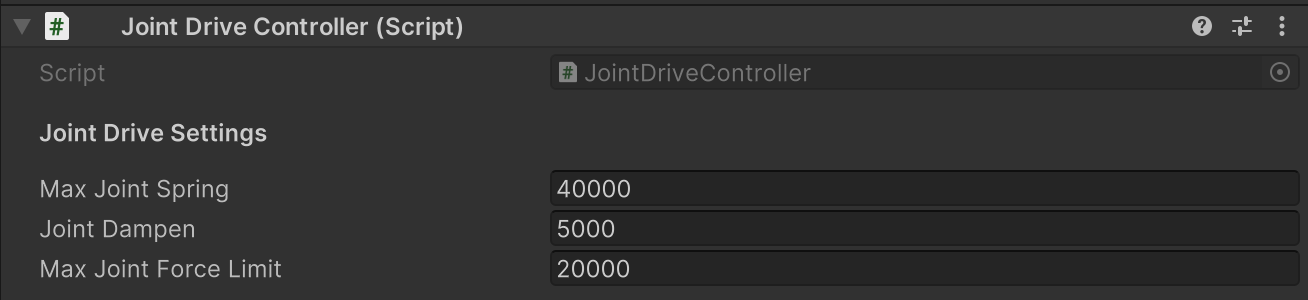
\includegraphics[scale=0.5]{img/gelenk_motor_steuerung.png}
  \caption{Gelenk Motor Steuerung}
  \label{fig:gelenk_motor_steuerung}
\end{figure}

\begin{itemize}
  \item Max Joint Spring: Bestimmt den Drehmoment mit welchem das Gelenk in die Zielposition rotiert wird.
  \item Joint Dampen: Verringert den Drehmoment proportional zur Differenz zwischen aktueller Geschwindigkeit und der Zielgeschwindigkeit. Verringert Schwingungen.
  \item Max Joint Force Limit: Gibt die maximale Kraft des Gelenks an (verhindert zu schnelle Bewegung bei großer Abweichung).
\end{itemize}

\begin{figure}[H]
  \centering  
  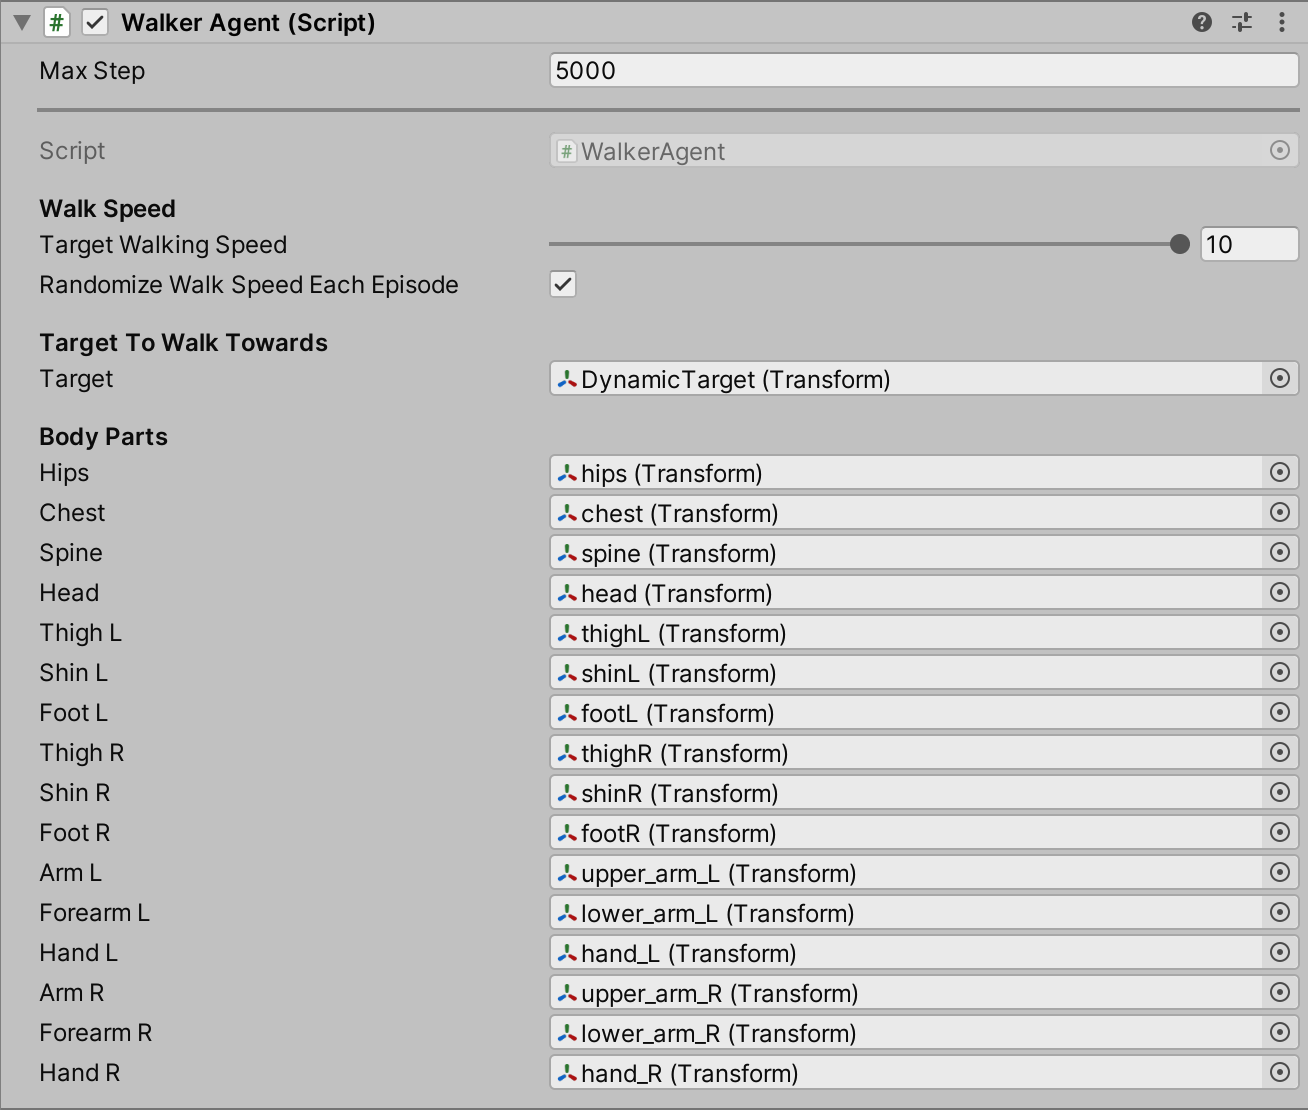
\includegraphics[scale=0.5]{img/agent_konfiguration.png}
  \caption{Agent Konfiguration}
  \label{fig:agent_konfiguration}
\end{figure}

\section{Training}

Zu beginn werden die Körperteile in der Gelenk Motor Steuerung initialisiert und das Ziel auf eine zufällige Position gesetzt.
Darauf folgend beginnt die Simulation der Trainingsepisoden. Hierfür werden alle Körperteile in ihre Startposition gesetzt und die Rotation des Läufers um die Y Achse zufällig gesetzt. Die zufällige Rotation hilf dabei das Verhalten des Läufers flexibel zu gestalten. Es wird weiterhin eine zufällige Zielgeschwindigkeit gewählt um zusätzliche Stabilität zu gewährleisten.

Sind die Vorbereitungen getroffen beginnt die Simulation mit einer Updatefrequenz von 75 Hz für die Phsikkalkulation. Der Agent fragt jedes fünfte Physikupdate eine Entscheidung an. Bei der Simulationsfrequenz von 75 Hz ergibt das eine Frequenz von 15 Anfragen pro Sekunde. Der Grund warum die Anfragen nur jedes fünfte Update angefragt werden ist das der Agent durch diese Einschränkung seine Bewegungen genauer wählen muss. Es kann so verhindert werden das der Agent zu hastige und ruckartige Bewegungswechsel lernt. Sobald eine Entscheidung angefragt ist, erfasst der Agent den Zustand der Umgebung. Dieser wird anschließend im referenzierten Verhalten ausgewertet und eine Aktion ausgewählt.

Die Beobachtung des Agenten wird in Tabelle \ref{table:walker_beobachtung} dargestellt. Für jedes Körperteil wird die Beobachtung aus Tabelle \ref{table:walker_beobachtung_körperteil} dem Zustand angefügt. Die Beobachtungen müssen den Zustand des Läufers und der Umgebung im Bezug auf das Trainingsziel genau darstellen. Nur so kann der Agent die Situation verstehen und eine passende Aktion auswählen und gleichermaßen sein Verhalten optimieren.

\begin{table}[H]
  \centering
  {\rowcolors{1}{gray!10}{white}
  \begin{tabular}{ |p{1cm}|p{9cm}|p{5cm}|}
  \hline
  \textbf{ID} & \textbf{Beobachtung} & \textbf{Anmerkung}  \\
  \hline
  \rowids & Abweichung Durchschnittsgeschwindigkeit von Zielgeschwindigkeit &  \\
  \hline
  \rowids & Durchschnittsgeschwindigkeit &  \\
  \hline
  \rowids & Zielgeschwindigkeit & \\
  \hline
  \rowids & Abweichung Hüftrotation von Zielrotation & \\
  \hline
  \rowids & Abweichung Kopfrotation von Zielrotation & \\
  \hline
  \rowids & Zielposition & \\
  \hline
  \rowids & Körperteil Beobachtungen & Beobachtung aus Tabelle \ref{table:walker_beobachtung_körperteil} für jedes Körperteil \\
  \hline
  \end{tabular}}
  \caption{Walker Agent Beobachtung}
  \label{table:walker_beobachtung}
\end{table}
\rowidsclear

\begin{table}[H]
  \centering
  {\rowcolors{1}{gray!10}{white}
  \begin{tabular}{ |p{1cm}|p{9cm}|p{5cm}|}
  \hline
  \textbf{ID} & \textbf{Beobachtung} & \textbf{Anmerkung}  \\
  \hline
  \rowids & Bodenkontakt & \\
  \hline
  \rowids & Geschwindigkeit & \\
  \hline
  \rowids & Rotationsgeschwindigkeit & \\
  \hline
  \rowids & Position relativ zur Hüfte & \\
  \hline
  \rowids & LokaleRotation & Fehlt für Hüfte und Hände \\
  \hline
  \rowids & Gelenkstärke & Fehlt für Hüfte und Hände \\
  \hline
  \end{tabular}}
  \caption{Walker Agent Körperteil Beobachtung}
  \label{table:walker_beobachtung_körperteil}
\end{table}
\rowidsclear

Das Format einer Aktion besteht aus den in Tabelle \ref{table:walker_aktion} aufgeführten Feldern für jedes Körperteil des Läufers, ausgenommen der Hüfte und Hände. Jedes Körperteil wird somit separat bewegt, um die Bewegungen zu optimieren und schlussendlich das Gleichgewicht zu halten und das Fortbewegen zu erlernen.

Die Hüfte ist das zentrale Körperteil woran alle weiteren Körperteile mit Gelenken direkt oder indirekt anknüpfen. Aufgrund dieser zentralen Rolle wird die Hüftbeugung über das Gelenk des verbundenen Körpers gesteuert.

Da die Hände kaum Relevanz für das laufen haben, sind in der Demo fest mit dem Unterarm verbunden und brauchen daher nicht gesteuert werden.

\begin{table}[H]
  \centering
  {\rowcolors{1}{gray!10}{white}
  \begin{tabular}{ |p{1cm}|p{9cm}|p{5cm}|}
  \hline
  \textbf{ID} & \textbf{Beobachtung} & \textbf{Anmerkung}  \\
  \hline
  \rowids & Rotationswinkel X & Nur wenn Körperteil X Rotation beweglich ist\\
  \hline
  \rowids & Rotationswinkel Y & Nur wenn Körperteil Y Rotation beweglich ist\\
  \hline
  \rowids & Rotationswinkel Z & Nur wenn Körperteil Z Rotation beweglich ist\\
  \hline
  \rowids & Gelenkstärke & \\
  \hline
  \end{tabular}}
  \caption{Walker Agent Aktion}
  \label{table:walker_aktion}
\end{table}
\rowidsclear

Nach dem Erhalten der Aktion werden über die Gelenk Motor Steuerung die Zielrotationen sowie die Maximale Kraft des Gelenks festgelegt, und somit der Läufer gesteuert.

Die Belohnungsfunktion enthält zwei Komponenten. Zum einen wird die Differenz der Bewegung in Zielrichtung zwischen momentaner Bewegung und Zielbewegung durch die Funktion $R_V$ bewertet. Somit wird der Läufer dazu motiviert effizient auf das Ziel zuzusteuern, indem Geschwindigkeit und Richtung optimiert werden. Zum Anderen wird die Abweichung zwischen momentaner Blickrichtung und der Zielrichtung in $R_L$ berechnet. Diese Komponente stellt sicher das der Läufer sich vorwärts geradeaus auf das Ziel bewegt. Die Belohnung ergibt sich am ende durch die Multiplikation beider Teilterme. Die Verwendung der Multiplikation hat zur Folge das die Belohnung gleichermaßen von beiden Teiltermen abhängig ist und es somit notwendig ist, beide Teile gleichzeitig zu optimieren. Als Ergebnis lernt der Läufer gleichermaßen die Ausrichtung als auch die Bewegung in Zielrichtung.

\begin{figure}[H]
  \centering  
  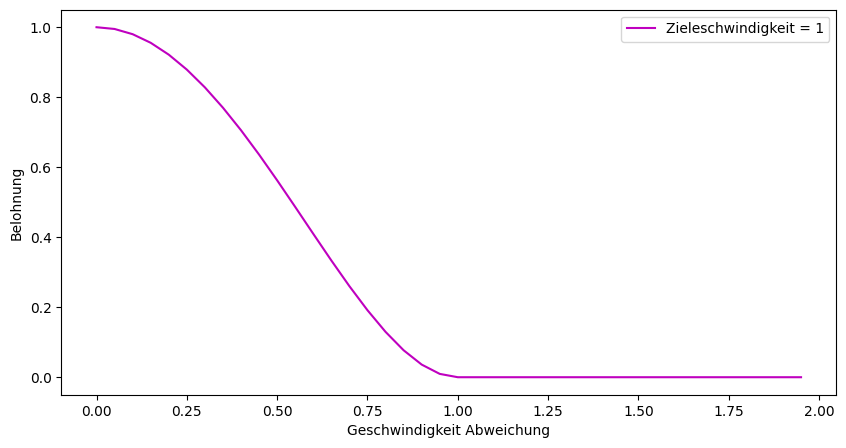
\includegraphics[scale=0.5]{img/match_velocity_demo_vel1.png}
  \caption{Walker Demo Match Velocity Belohnungsfunktion}
  \label{fig:match_velocity_demo_vel1}
\end{figure}

$V_\delta=Clip(|\vec{Geschwindigkeit} - \vec{Zielgeschwindigkeit}|, 0, |\vec{Zielgeschwindigkeit}|)$ \\
$R_V=(1 - (V_\delta / |\vec{Zielgeschwindigkeit}|)^2)^2$ \\

\begin{figure}[H]
  \centering  
  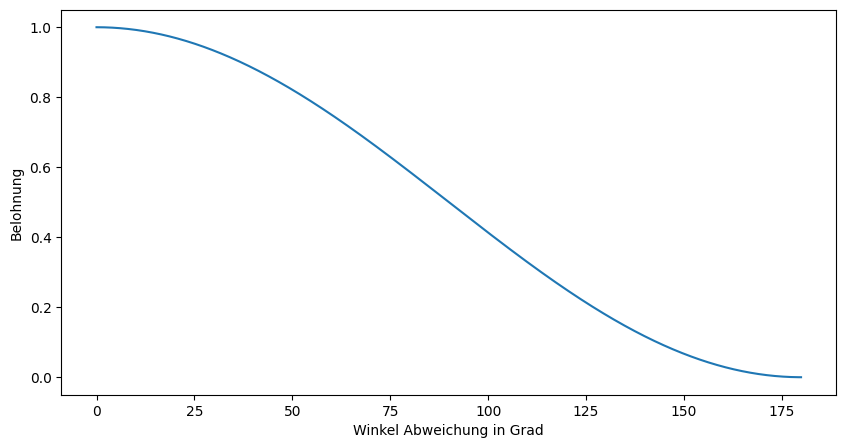
\includegraphics[scale=0.5]{img/look_at_target_demo.png}
  \caption{Walker Demo Look At Target Belohnungsfunktion}
  \label{fig:look_at_target_demo}
\end{figure}

$R_L=(\vec{Zielrichtung} \cdot \vec{Blickrichtung})+ 1) \cdot 0.5$ \\
$R=R_V \cdot R_L$

Die Belohnung wird in jedem Physikupdate neu berechnet und dem Agenten hinzugefügt. Die Belohnung wird für den Zeitraum zwischen zwei Entscheidungen aufsummiert. Bevor die nächste Entscheidung getroffen wird, wird das Tupel aus Beobachtung, Aktion und erhaltene Belohnung im Trainingsbuffer gespeichert. Hat der Buffer genug Informationen gespeichert beginnt ein Lernprozess in welchem die zuvor gespeicherten Tupel evaluiert werden. Es wird der PPO Algorithmus auf Teilbatches ausgeführt und so schrittweise das Verhalten angepasst.

Erreicht der Läufer ein Ziel wird dieses an eine neue zufällige Position in der Umgebung bewegt.

Die Trainingsepisode läuft solange bis entweder 5000 Schritte erreicht sind oder der Läufer fällt. Wenn ein Körperteil des Läufers, ausgenommen den Füßen und Schienbeinen, den Boden berührt wird die Trainingsepisode sofort beendet. Diese Technik nennt man frühes stoppen, es wird verwendet um zu verhindern das der Agent einen Großteil des Trainings in zuständen verbringt welche für das eigentliche Ziel keinen Mehrwert bieten. Fällt der Läufer benötigt es eine sehr komplexe Reihenfolge an Aktionen zum zurück auf die Beine zu kommen. Im Ende bringt es den Läufer aber kein bisschen weiter an das eigentliche Ziel. Ist die Episode zu Ende wird sofort eine neue gestartet.

\section{Auswertung}
Der Agent der Walker Demo erlernt über 30 Millionen Trainingsschritte ein Verhalten welches beinahe die Grenze der Episodenlänge erreicht ohne zu fallen. Dabei erreicht es zudem eine durchschnittliche Belohnung pro Episode von 1600 (siehe Abbildung \ref{fig:analyse_training}). Die durchschnittliche Belohnung ist ohne Kontext erstmal nur eine Zahl. Schaut man jedoch genauer ergibt sich die durchschnittliche Belohnung aus der durchschnittlichen Episodenlänge angegeben mit der Anzahl an angefragten Entscheidungen. Mit 800 Anfragen pro Episode kommt man auf 4000 Trainingsschritte beziehungsweise Physikupdates. Teilt man nur die durchschnittliche Belohnung mit der Anzahl an Schritten kommt man auf eine durchschnittliche Belohnung von ca. 0.4 pro Schritt. Die im Verlauf der Arbeit hinzugefügten Statistiken der Belohnungen zeigen eine Aufteilung von 0.9 Belohnung für die Blickrichtung und 0.45 für das halten der Zielgeschwindigkeit (siehe Abbildung \ref{fig:analyse_training_belohnung}. Eine Belohnung von 0.9 der Blickrichtungsbelohnung ergibt eine Abweichung von durchschnittliche 35 Grad. Die Zielgeschwindigkeitsbelohnung ergibt eine Abweichung von ca. 51\%.

\begin{figure}[H]
  \centering  
  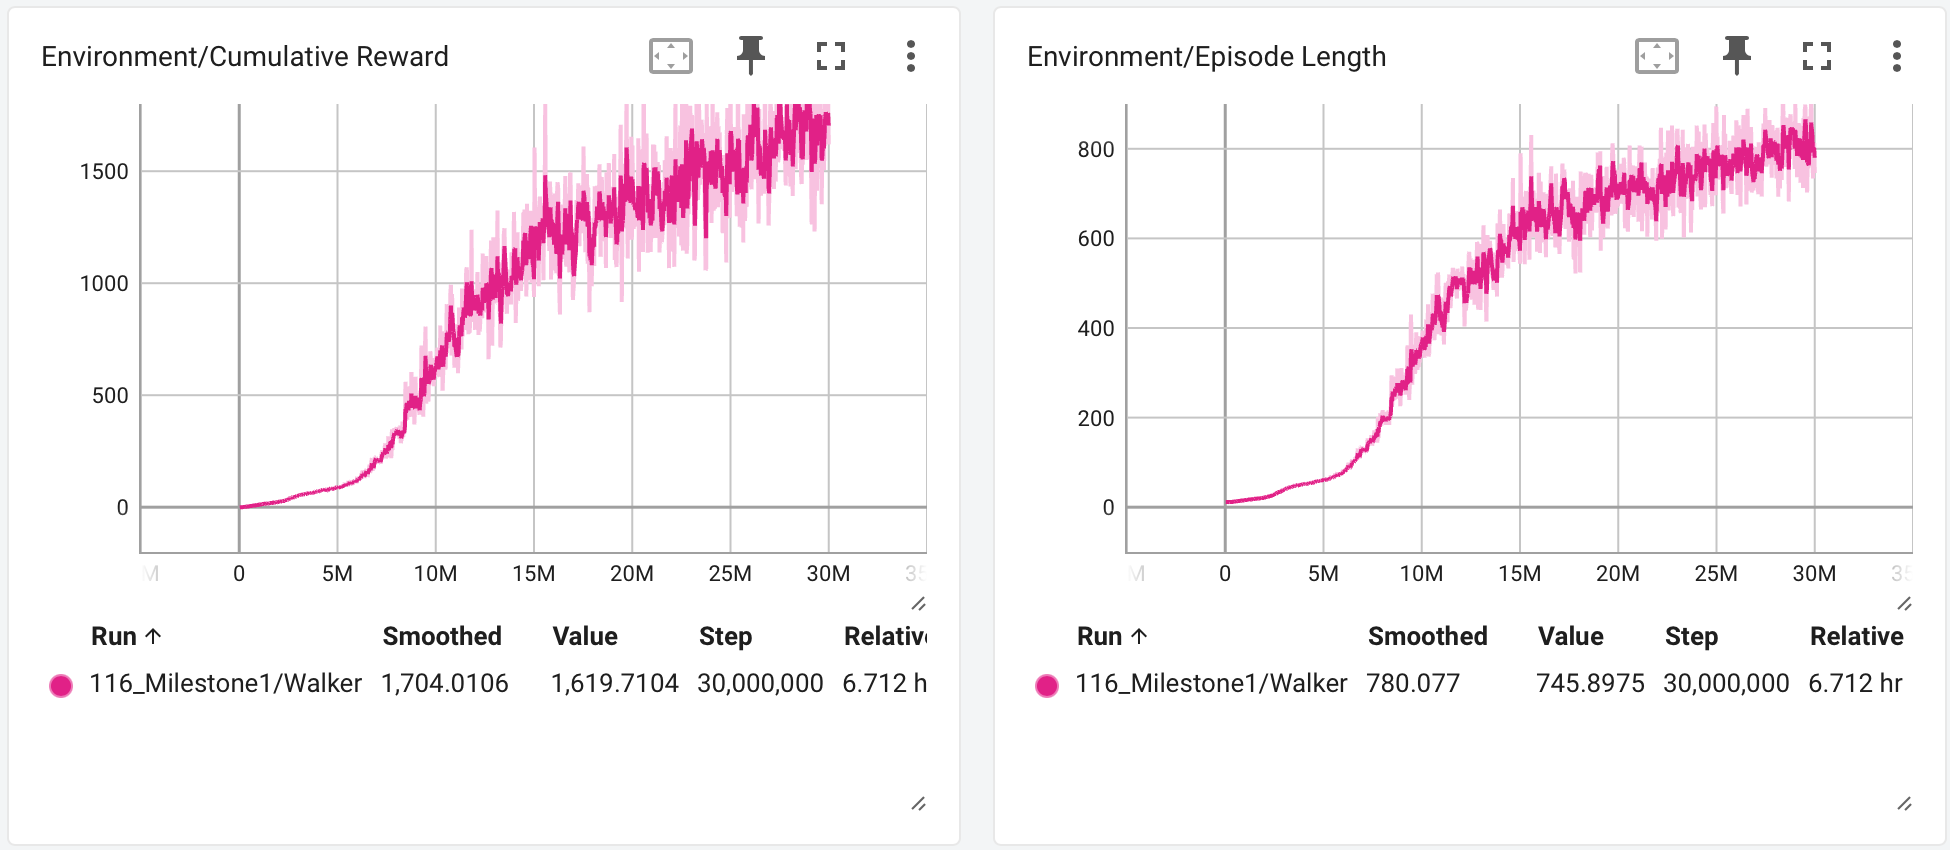
\includegraphics[scale=0.5]{img/analyse_training.png}
  \caption{Walker Demo Analyse Trainingsgraphen}
  \label{fig:analyse_training}
\end{figure}

\begin{figure}[H]
  \centering  
  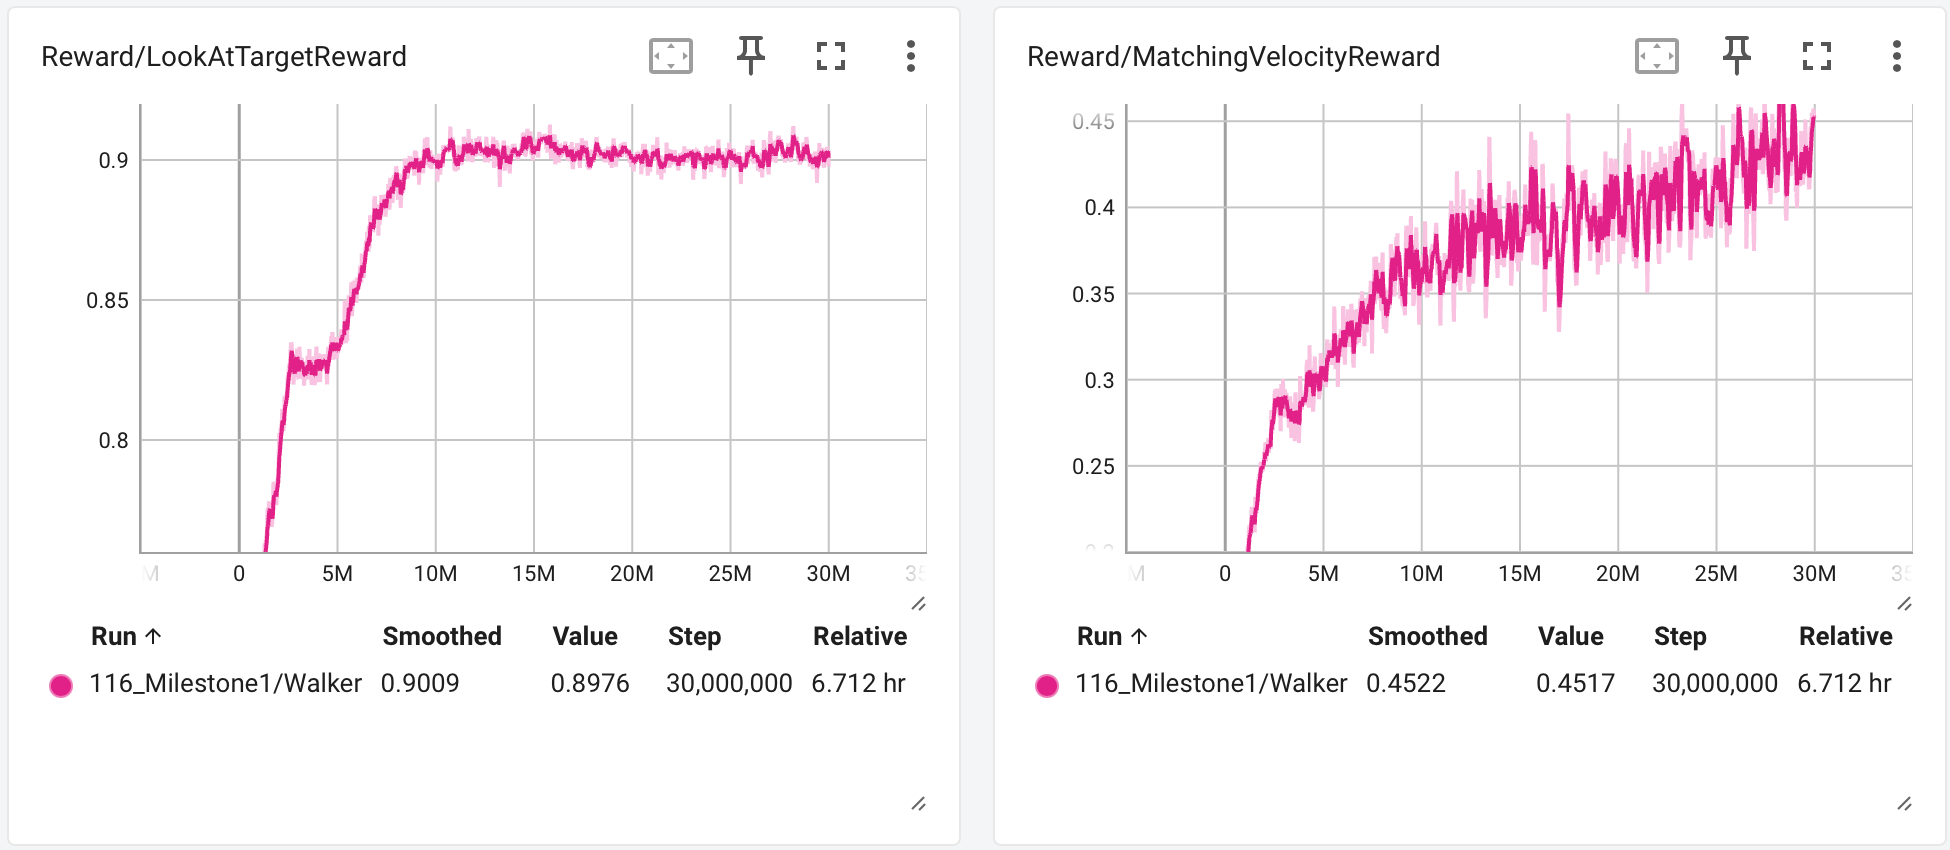
\includegraphics[scale=0.5]{img/analyse_training_belohnung.png}
  \caption{Walker Demo Analyse Training Belohnungsgraphen}
  \label{fig:analyse_training_belohnung}
\end{figure}

\begin{figure}[H]
  \centering  
  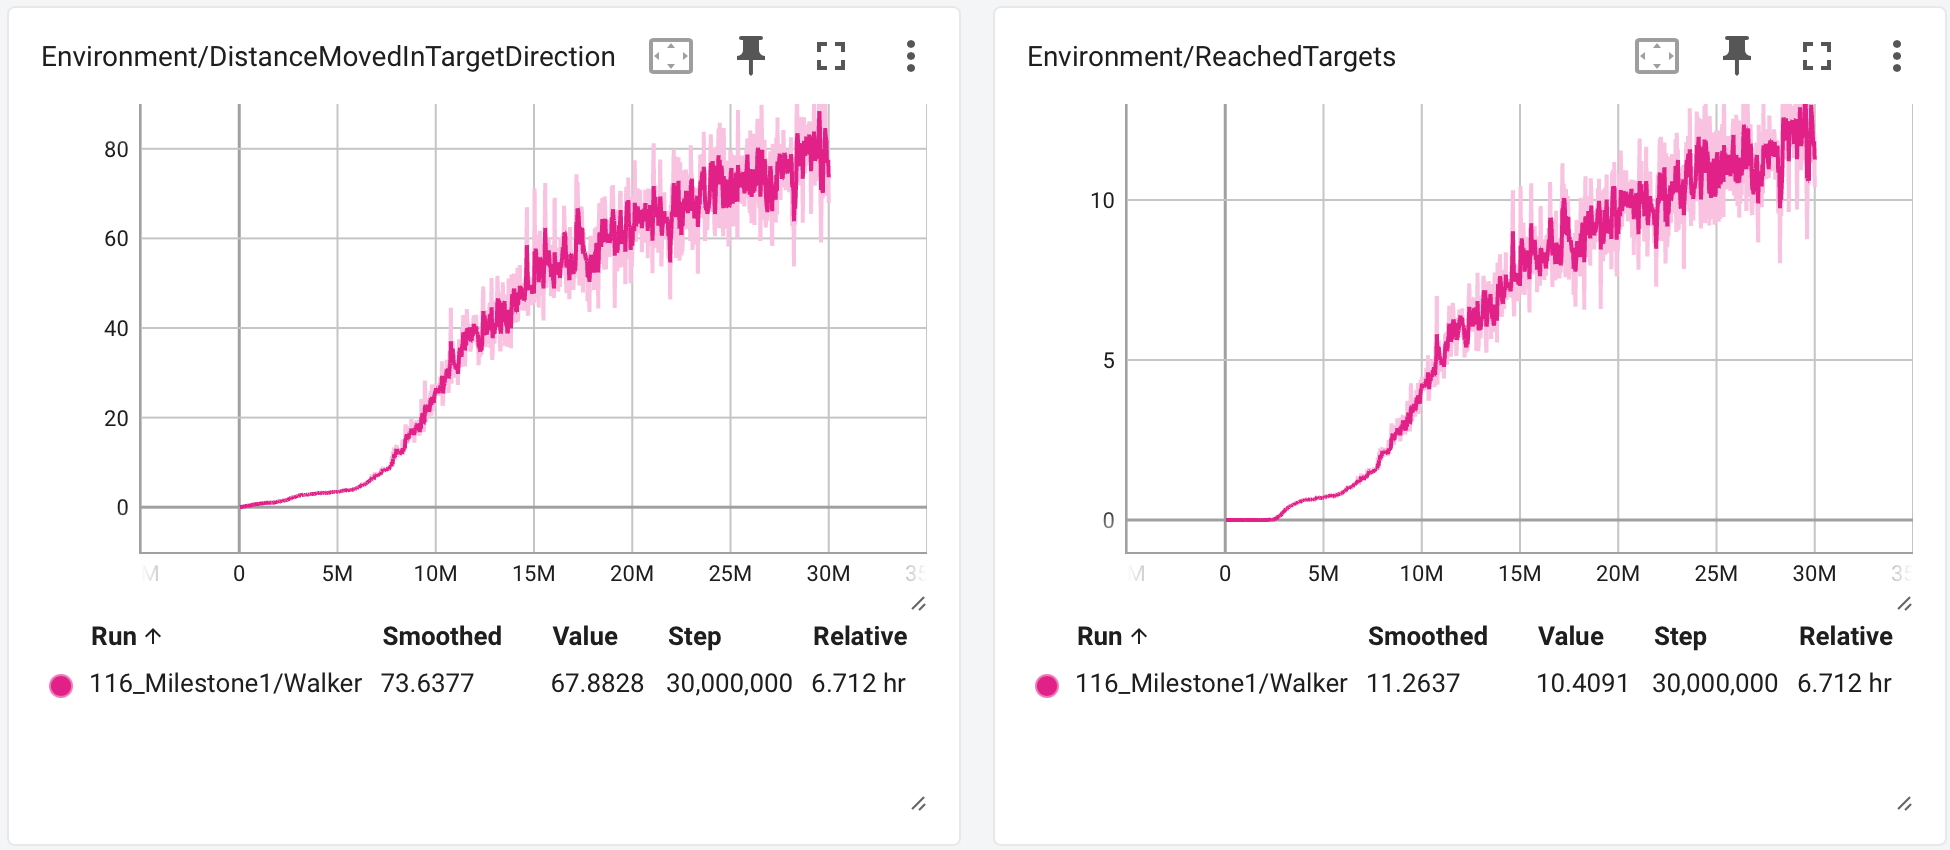
\includegraphics[scale=0.5]{img/analyse_training2.png}
  \caption{Walker Demo Analyse Training Zielgraphen}
  \label{fig:analyse_training_2}
\end{figure}

Der Läufer lernt nicht die Belohnungen bis zum Limit auszureizen, aber wie in Abbildung \ref{fig:analyse_training_2} zu sehen läuft er während einer Episode durchschnittlich eine Distanz von 80 Einheiten und erreicht dabei 10.4 Ziele.